%------------------------------------------------
\section{Introduction}
%------------------------------------------------
\begin{frame}[t]
	\frametitle{Background: COVID-19 forecasting targets}
	\tikzstyle{background grid}=[draw, black!50,step=.5cm]
	%
	Forecasting novel epidemics is a multidisciplinary field involving multiple \emph{targets} \footpartcite{Wu2021}\\
	\emph{Inputs} for forecasting \emphasis{epidemic size:}\\
    %
    \begin{itemize}
        \item<2-> Growth rate indicators
        \item<3-> \only<5->{\emphasis}{Historical incidence rate data}
        \item<4-> \only<5->{\emphasis}{Serologic assays}\\
        \centering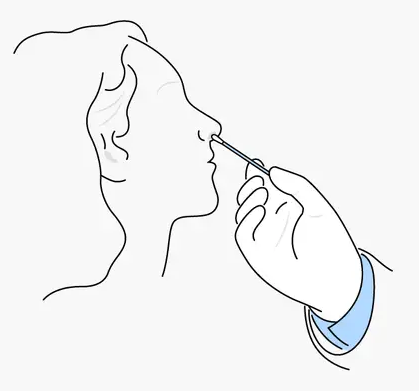
\includegraphics[width=0.23\textwidth]{targets/pcr.png}
    \end{itemize}
    %
	\tikzstyle{background grid}=[draw, black!50,step=.5cm]
	\begin{tikzpicture}[remember picture, overlay] %show background grid, 
		% Put the graphic inside a node. This makes it easy to place the
		% graphic and to draw on top of it. 
		% The above right option is used to place the lower left corner
		% of the image at the (0,0) coordinate. 
		\node [inner sep=0pt,above left, opacity=1.0]  at (0.99\textwidth,-0.0\textheight) (seq2seq) 
			{
				\only<1>{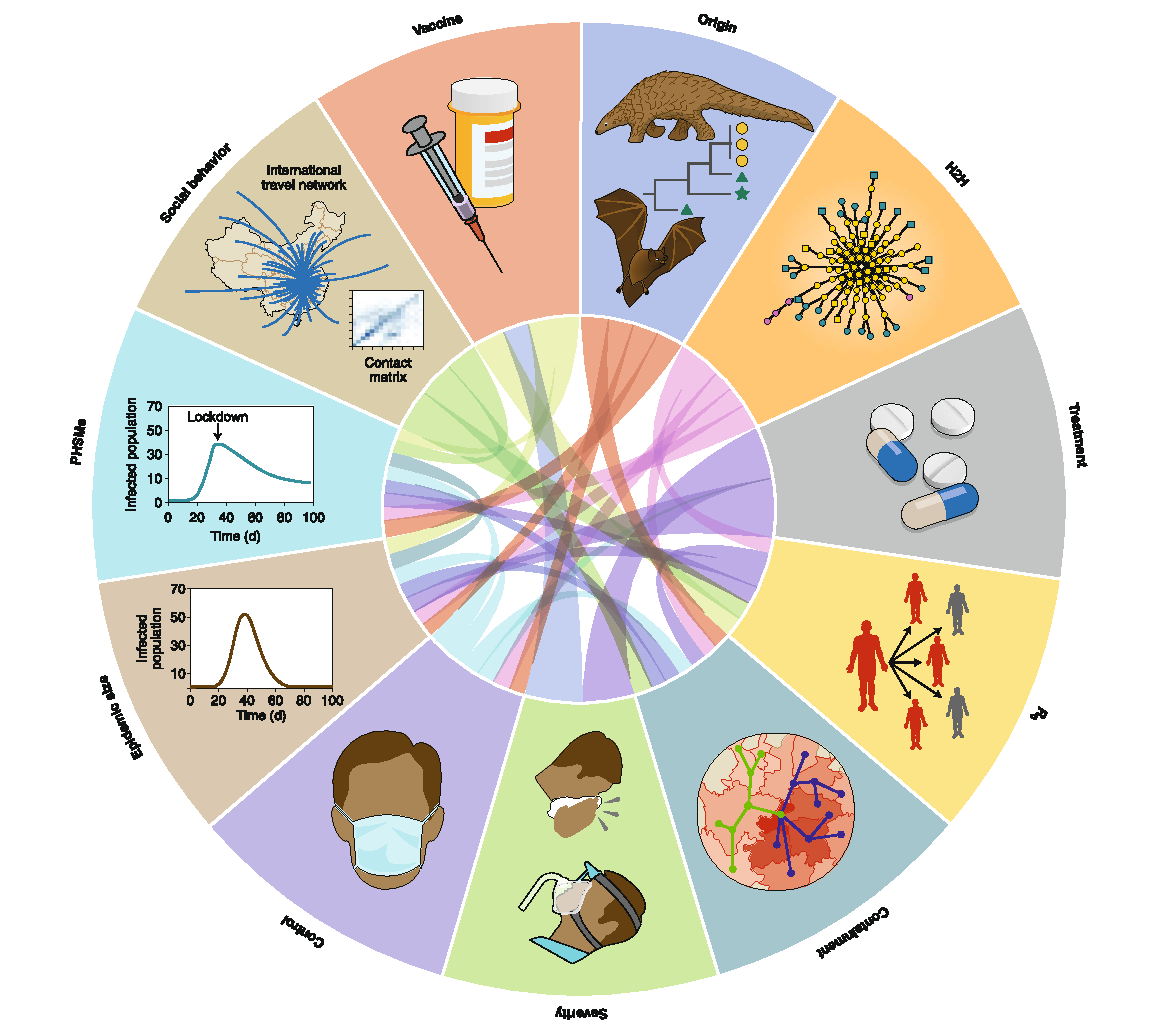
\includegraphics[width=0.45\textwidth]{targets/nowcasting_targets_1.pdf}}%
				\only<2>{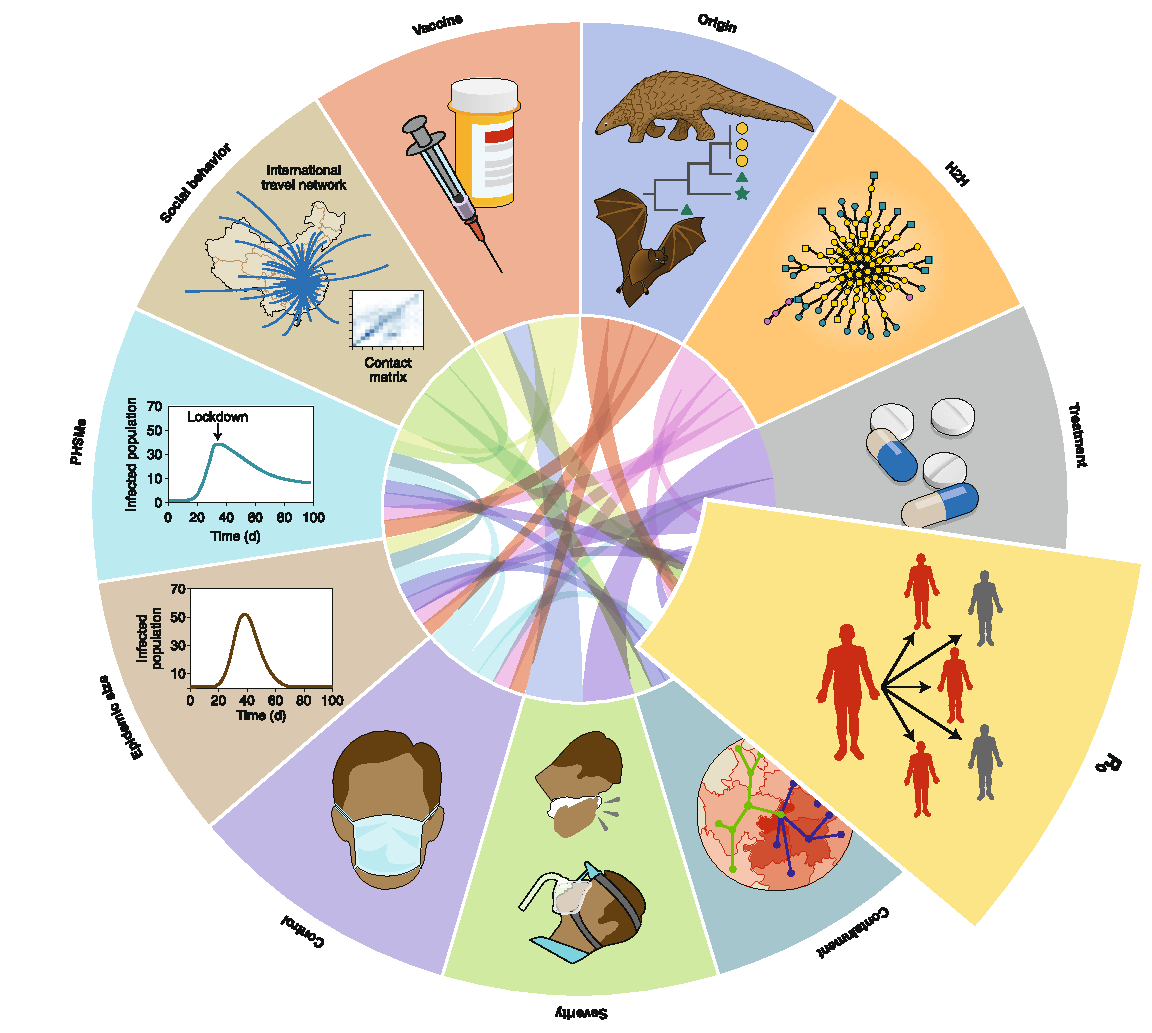
\includegraphics[width=0.45\textwidth]{targets/nowcasting_targets_2.pdf}}%
                \only<3->{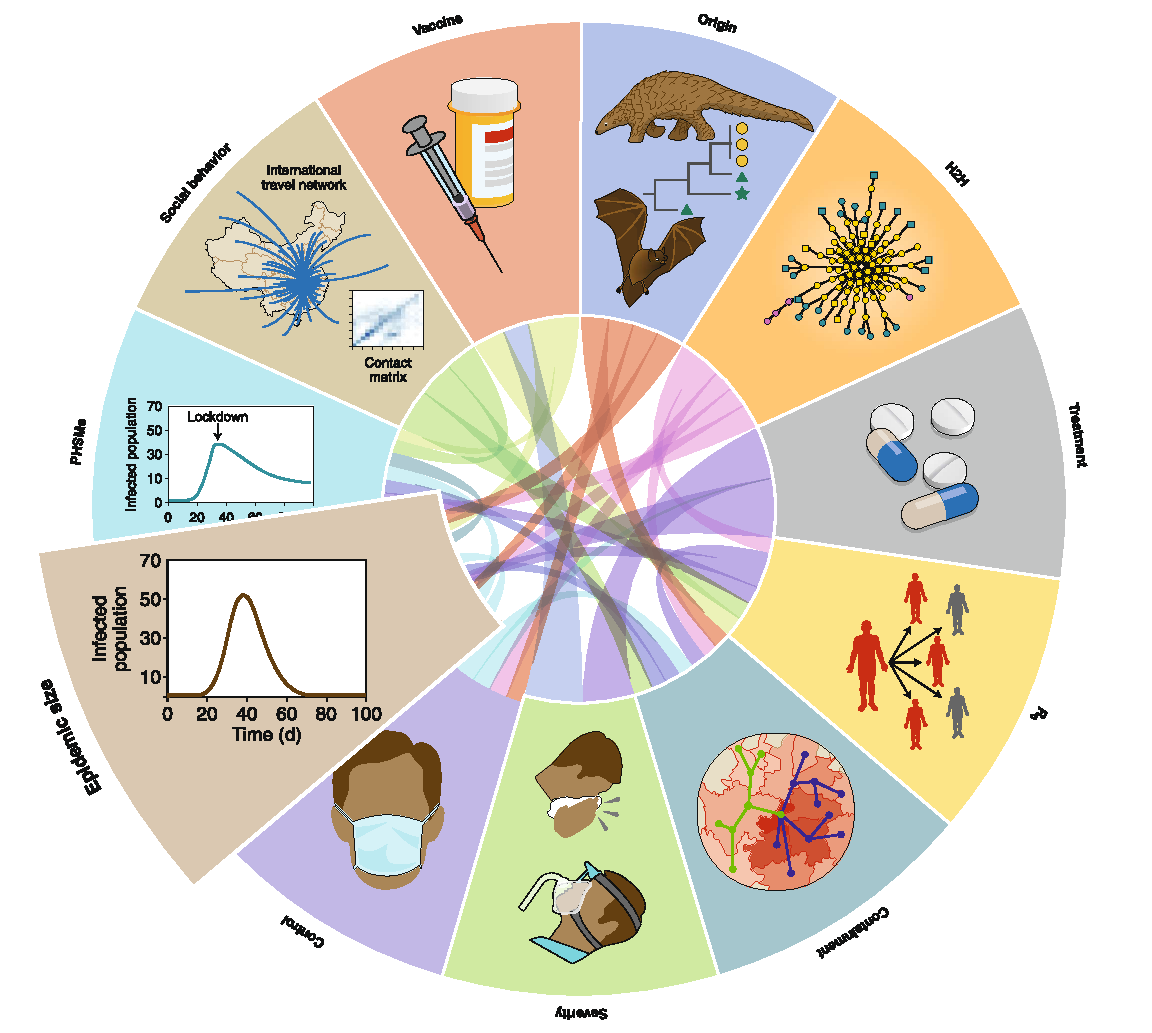
\includegraphics[width=0.45\textwidth]{targets/nowcasting_targets_3.pdf}}%
			};
		\only<1->{
			\node[inner sep=0pt,below=\belowcaptionskip of seq2seq,text width=\linewidth]
				{\vspace{-1em}{Nowcasting targets}};
		}%
		% show origin
		% \fill (0,0) circle (2pt);
	\end{tikzpicture}%
	%
	\vspace{-3em}
\end{frame}
\addtocounter{footnote}{-1}
%------------------------------------------------